
\section{Introduction}

\subsection{Project description}

The project is to implement a serializer from Haskell to an intermediate
format using GHC, and a deserializer from the intermediate format to an
interpreter usin PyPy. And then to test the result on some simple Haskell
programs. The hope is that this can serve as a base for future development
into a full Haskell JIT compiler.

\subsection{Motivation}

The motivation behind the project is to see if a \emph{strongly-typed} 
\emph{non-strict} \emph{purely-functional} programming language, Haskell, 
can benefit from just-in-time (JIT) compilation.

Some people seem to think that there is little to gain from using 
JIT compilation of statically typed languages since they can be
so heavily optimized at compile time. However, a JIT compiler has a lot
more information to work with.

PyPy is a project that implements a meta-tracing JIT. The project
defines a proper subset of Python called RPython. This language has 
the characteristics that it is possible to perform type-inference on it.
The idea is that interpreters can be written rapidly in RPython, and the
interpreter implemented in RPython will benefit from PyPy's JIT compiler.
To optimize the interpreter, the RPython toolchain accepts some compiler
hints to determine what parts of the code to trace, and to define the 
static and dynamic parts of the interpreter "memory".

GHC (Glasgow Haskell Compiler) is the most advanced compiler for the
Haskell programming language. The GHC team has defined an external format
of Haskell called \emph{External Core}. GHC's front-end translates
Haskell 98 (plus some extensions) into Core. This way it is possible to
reuse GHC for parsing, desugaring and typechecking, while implementing
the back-end separately. \cite{tolmach2010ghc}

\subsection{System description}

The system will use the GHC Haskell library to generate the 
representation of the Core language and a simple Haskell program to 
serialize this representation into JSON. This entails using GHC for
parsing, typechecking, desugaring and simplification. Simplification
is an optimization step in GHC, performing small and simple transformations.

The resulting code will then be deserialized by the PyPy Haskell interpreter 
and executed. See figure \ref{overview} for a description of the implemented and
to-be-implemented parts of the project.

\begin{figure}[H]
\centering
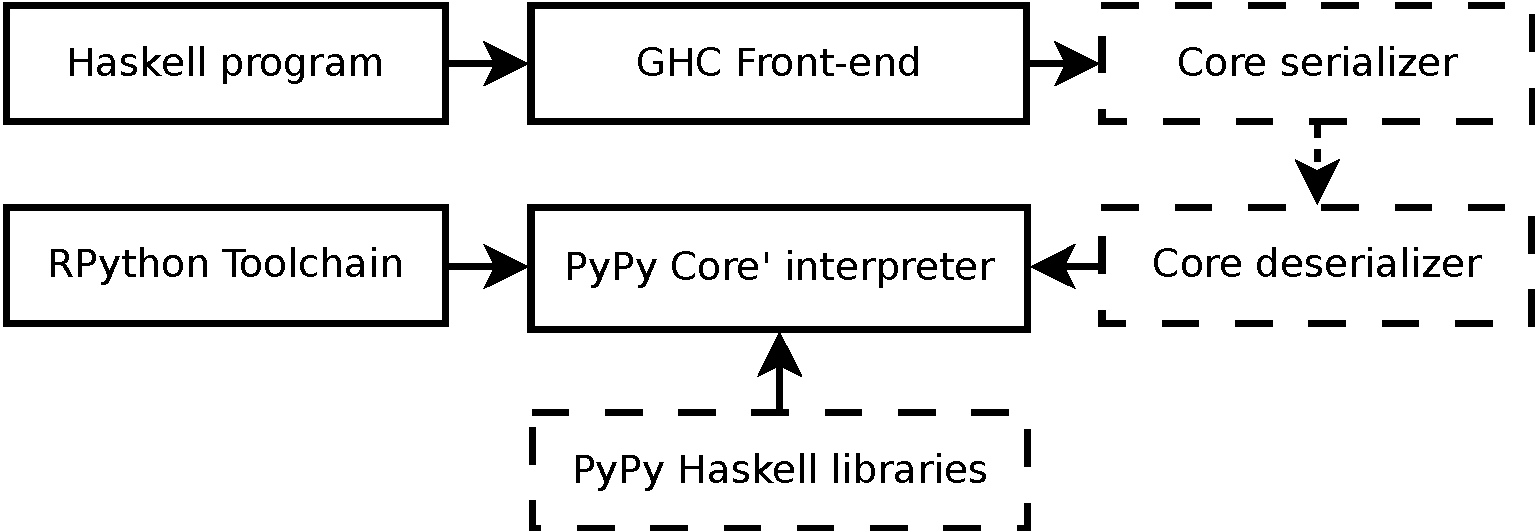
\includegraphics[width=0.8\textwidth]{diags/overview}
\caption{Project overview. Full border: implemented, Dotted border: unimplemented.}
\label{overview}
\end{figure}

\subsection{Structure of the paper}

Follwing this introduction is a section (Section 3: Background) discussing the 
background of the project. The background section contains some information about 
the tools beeing used, and why.
Section 3 (External-core) contains a description of the external language representation
of the intermediate language used by GHC.
Section 4 (JSON representation of Core) follows with the description of the intermediate format
used in this project, which is a combination of JSON and external-core.
Section 5 (Implementation) discusses the implementation of the system, the issues faced
during development and some of the remaining issues.
In section 6 (Examples), example programs are passed through the pipeline with intermediate
representations presented at each step.
Section 7 (Future Work) discusses work to be done in the future.


